%%%%%%%%%%%%%%%%%%%%%%%%%%%%%%%%%%%%%%%%%%
\chapter{Theoretical Framework}
\label{sec: theory}
\markboth{}{Theoretical Framework}
\epigraph{\emph{In actual experience, there is never any such isolated singular object or event; an object or event is always a special part, phase, or aspect, of an environing experienced world—a situation’}}{\citep[p. 67]{dewey1934}}

In the previous chapter, I outlined the increasing use of AR as a medium for the creation of meaningful experiences through interactive artwork. Examining the application of “real-time computationally mediated perception” \citep{kiefer2018} as a definition for AR, this chapter considers a trio of theoretical lenses through which to consider this process of mediation and the types of aesthetic experience this results in. Namely, I will consider the material, embodied, and spatial relations that AR fosters within this context of artistic production and experience.



%%%%%%%%%%%%%%%%%%%%%%%%%%%%%%%%%%%%%%%%%%
\section{Knowledge and Aesthetic Experience}\label{sec: theory-aestheticexperience}
What is experience when it comes to art; how does it relate to epistemological practice? To address this question, the present thesis draws from the work of the American pragmatist John Dewey (1859-1952). In his 1934 text, Art as Experience, Dewey argues that the production and consumption of art faces a crisis. After having been historically coupled in an constitutive relationship with the processes of everyday sociocultural life, it is being increasingly separated from these “conditions of origin and operation in experience” \citep{dewey1934}, in a way that places art upon a remote pedestal. Dewey describes this as a product of the growth of capitalism. On proposing what they term Dewey Aesthetics, Leddy and Puolakka write:
\begin{quote}
    “Nothing about machine production per se makes worker satisfaction impossible. It is private control of forces of production for private gain that impoverishes our lives. When art is merely the ‘beauty parlor of civilization,’ both art and civilization are insecure. We can only organize the proletariat into the social system via a revolution that affects the imagination and emotions of [hu]man[kind]. Art is not secure until the proletariat are free in their productive activity and until they can enjoy the fruits of their labor. To do this, the material of art should be drawn from all sources, and art should be accessible to all.” \citep{leddy2021}
\end{quote}
From this standpoint, art can serve as an emancipatory force for positive social change; but only on the condition that it is first brought back to the “origin and operation” of everyday experience — through the democratisation of a wider corpus of artistic media, tools, and social contexts in which these are deployed. In the 21st century, we could mistake this for already having happened. The increasing availability of ubiquitous technologies such as the internet, wearables, smartphones, powerful computers and software have shifted artistic production closer to the site of everyday sociocultural life — from the studio to the bedroom. Yet in doing so, has art really been knocked from its pedestal and been re-integrated into, and resituated to arise from everyday life? 

Today, the fabric through which art tends to be disseminated and therefore consumed, social media, arguably operates within this same capitalist framework, the vocabulary having shifted from art in the museum, to content on our feeds. Despite making art more accessible to produce and consume, the capitalist logic of surplus extraction the centre of the algorithms that determine our interaction with social media vies to keeps art separate from everyday life. Central to this is that instead of being centralised in a museum or gallery, it is the concept of the pedestal itself that we should venerate. We must each curate our own museums and galleries, our own feeds.

The unavoidable truth of these platforms however, is that they are not solely focused on fostering individual or even collective curation of democratised art/content. They still employ the capitalist framework at their core. This extractivist profit motive defines the algorithmic fabric of online “content creation” (production), and resultant social media “engagement“ (consumption) through mass data harvesting and advertisement selling. The longer users are engaged on a platform (Facebook, Instagram, Twitter, YouTube, TikTok), the more likely they are to generate profits for the platform via advert click/tap-throughs. Our feeds are interspersed with adverts and sponsored posts that have been carefully curated to maximise the potential click/tap-through rate of their victims. Soshana Zuboff defines this as arising from a “market of human behavioural futures” [p?] in her book Surveillance Capitalism. Through this surveillance, large amounts of behavioural/affectual/personal data (termed behavioural surplus by Zuboff) are ‘skimmed’ off the top of our engagement with these platforms, and sold to agencies that match this personal data with products/content you are most likely to engage with. How could it be argued that that the production and consumption of art / content on such platforms is not governed by “private gain” at our expense? 

More recently, there are facets of the rise of NFT art projects that epitomise this continued fetishisation and veneration of digital fine art under the guise of “decentralisation”. Unfortunately enough, these projects often fall foul to the exact “centralisation” they market to oppose, creating small micro-communities of inter-centralised followers that collectively and actively, through social media, ensnare new and uninitiated retail investors via the urgency phenomenon of the “fear of missing out”. The motivation being to increase the value of their own NFTs. In most NFT projects, the only drive is profit motive, the digital art is merely the vehicle through which this investment is (im)materially realised. Despite the technological basis of some of these projects being quite radical in their proposition of democratic ownership and the privacy and security of digital information, the asset class most of them end up facilitating is tied to a pyramid scheme that necessitates the enrichment of the creators and early adopters of that specific NFT collection. How, in any way, could this method of production and consumption be said to be different from Dewey’s outlining of the rise of the “nouveaux riches”:
\begin{quote}
    “The nouveaux riches, who are an important byproduct of the capitalist system, have felt especially bound to surround themselves with works of fine art which, being rare, are also costly. Generally speaking, the typical collector is the typical capitalist. For evidence of good standing in the realm of higher culture, he amasses paintings, statuary, and artistic bijoux, as his stocks and bonds certify to his standing in the economic world.” \citeyearpar[p. 7]{dewey1934}
\end{quote}
It could be argued therefore, that we have witnessed an increase in the amount of new media formats, but not one that resituates production outside of capitalist logic for the masses; even in so called “decentralised” projects. When Leddy and Puolakka stress that it is this “private control of [the] forces of production for private gain” that leads to this disconnection of art from experience, it follows that the creation of art outside of the confines of this control addresses the imperative for the drawing of art “from all sources” [own emphasis]. From this view, the convergence of digital art to their “conditions of origin and operation in experience” could be seen as one of the primary foci of more recent movements such as Maker, Hacker, and DIY Labs, as well as the general ethos of participatory design and open-source hardware and software in art, design, and electronic music practice.

But what does it mean to say that art ought to originate and operate “in” experience, and how might these movements address this? Dewey considers the “live creature” in response to this question. He views the participant of aesthetic experience as meaningfully inseparable from the environment in which they are embedded: 
\begin{quote}
    “The senses are the organs through which the live creature participates directly in the on-goings of the world about [them]. In this participation the varied wonder and splendour of this world are made actual for [them] in the qualities [they experience]. This material cannot be opposed to action, for motor apparatus and “will” itself are the means by which this participation is carried on and directed. It cannot be opposed to “intellect”, for mind is the means by which participation is rendered fruitful through sense; by which meanings and values are extracted, retained, and put to further service in the intercourse of the live creature with [their] surroundings.” \citeyearpar[p. 22]{dewey1934}
\end{quote}
From this basis, namely that perception, sensorimotor action, and intellect cannot be meaningfully separated when considering the intercourse of participants with their environment, Dewey highlights the weakness in the traditional dualist theory of mind -  we are embodied and embedded beings. He posits that experience results from the “interaction of organism and environment”,  and that in its fullest, experience can represent a “transformation of interaction into participation and communication”. It would follow, therefore, that in the production of artistic works, consideration of this dynamical relationship that constitutes our subjective experiences is not only valuable, but that artistic works should aim to arise (originate) from common and relatable states of this relationship.  Returning art to this origination and operation “in” experience through interactive and participatory digital means can therefore be seen as a crucial mechanism for inducing positive societal change through fostering new channels of “participation and communication”. Shifting the production of artistic work away from the exploitative practices of mass manufacturing inherent in consumer technologies, as well as centring embodied participatory design practices, is a common theme among DIY and Makerspace communities.% The labour involved in the production of free and open source software and hardware is often what enables this, and will be expanded upon in the next chapter. 

This is not to in any way demean or reduce the social importance of art that does not take these approaches. It is also especially tricky to prove in any certainty the subjective measures of aesthetic experience that could result in positive societal change. However, I do view the imperative to shift production and consumption of art outside the capitalist architecture of current proprietary software tools and consumer technologies, and bringing the aesthetic closer to every day experience as a fruitful endeavour for the artist. I argue that doing so would emphasise the dynamical relationship participants find themselves in with their and, crucially, others’ sociocultural, economic, and ecological contexts.

Where does knowledge lie for us as researchers in the production and consumption of such artistic works? On what basis can we test and evaluate these claims? One view that is popular in the field of music technology is that of considering the nature of the interactive and digital systems that we develop; a consideration of the epistemic tool. 
\begin{quote}
    “The digital instrument is an artefact primarily based on rational foundations, and, as a tool yielding hermeneutic relations, it is characterised by its origins in a specific culture. This portrayal highlights the strengthened responsibilities on the designers of digital tools, in terms of aesthetics and cultural influence, as they are more symbolic and of compositional pertinence than our physical tools.” \citep[p. 335]{magnusson2009a} 
\end{quote}
Developed by Magnusson, this line of thinking proposes that the digital instruments we design and employ as artists have inscribed in their physicality, affordance and sonic output, knowledge of cultural, historical, and designerly significance. In this way, they can be considered complex systems of research importance through the examination of their symbolic design, construction, performance, and appreciation by audiences. Magnusson embeds this proposition within Don Ihde’s philosophy of ‘instrumental realism’ and Wittgenstinian philosophy, and draws from an understanding of the extended mind hypothesis. This theory, which will be expanded on in the next section, proposes that 
\begin{quote}
    “[Under certain conditions], the human organism is linked with an external entity in a two-way interaction, creating a coupled system that can be seen as a cognitive system in its own right.” \citep[p. 7]{clark1998}
\end{quote}
Similar to Dewey’s conception of how the live creature is inseparable from the environmental conditions that it is embedded in, the extended mind hypothesis and similar theories of embodied cognition prove to be invaluable in the field of tangible user interfaces, and digital music instrument design, due to the way they can explicate as well as draw out the dynamic relationships between artist, collaborator, material, interface, and audience in the deployment of expressive artistic media. In the following sections, I shall dive deeper into these theories of mind (ToM), and what they have to offer a practice that makes use of augmented reality technologies within the field of computational art and musical performance.



%%%%%%%%%%%%%%%%%%%%%%%%%%%%%%%%%%%%%%%%%%
\section{The 4E Approach to Experience}\label{sec: theory-4e}
One way of expanding on this conception of aesthetic experience is to adopt the 4E approach to cognition and experience. Key to my following theoretical underpinning of materiality, embodiment, and space will involve how this approaches the themes of perception, agency and cognition arising through the complex interthreaded coupling between a participant and their environment. Often referred to as 4E cognition (4EC), it states that cognition is an embodied, embedded, enactive, and extended process \citep{gallagher2017}. It’s worth mentioning that 4EC is an amalgam of related theories of mind (ToM) across the disciplines of philosophy and the social and cognitive sciences, and as such there are different flavours of it. Many of these have said to have roots in the Dewey’s pragmatism (among others’) outlined in the previous section, as well as Merleau-Ponty’s embodiment theories \citep{zavota2016}. What these constituent theories all bear in common is the rejection of the standard cognitivist model of experience that states that cognitive processes happen solely ‘in the mind’ and ’in the brain’. Another principle is that they generally draw from complex systems theory: “understanding the complex interplay of brain, body and world requires the tools and methods of nonlinear dynamical systems theory” \citep{clark1999}. Within this theory there are a multitude of phenomena that can explicate the interactions between components of such a continually unfolding system, including \citep{dedomenico2019}:
\begin{itemize}
    \item Interactions - a complex system is formed of many components, many of which will be connected in a network of mutual and on-going interaction
    \item Emergence - from this network of interactions, there exists the possibility for complex and novel structures to form that are inexplicable from the features of their simpler components 
    \item Dynamics - the state of a complex system can change over time, often in an unpredictable non-linear fashion
    \item Self-organisation - the components of a complex system may exhibit collective behaviours, and perceived large scale structure
    \item Adaptation - complex systems don’t necessarily shift between steady states, they actively and reactively respond to environmental stimuli
    \item Feedback - structures of a complex system exhibit a phenomena where the outputs of a system are routed back in, via closed chains of cause and effect 
\end{itemize}

4EC normally begins with an acknowledgement of the complex embodied nature of human cognition. Varela, Thompson, and Rosch propose that cognition is embodied in a way not too dissimilar to the assertion Dewey holds in regards to the “senses” of the “live creature”.
\begin{quote}
    “By using the term embodied we mean to highlight two points: first, that cognition depends upon the kinds of experience that come from having a body with various sensorimotor capacities, and second, that these individual sensorimotor capacities are themselves embedded in a more encompassing biological, psychological, and cultural context.” \citeyearpar[pp. 172-173]{varela1993}
\end{quote}
Alva Nöe’s concept of sensorimotor contingencies has since built on the first point of this approach to embodiment, in a way that proposes an “enactive approach to perception” accepts that perception is something we do, not something that happens to us \citep{noe2004}. This has since been termed the ‘sensorimotor approach’ to enactivism, and Gallagher notes that it falls short of an “enactivist approach” due to its omission of affective aspects of embodiment such as “mood-related and emotional factors, […] bodily states such as hunger, fatigue, and pain, as well as a complex motivational dimension that animates body-world interaction”  \citep[p. 150]{gallagher2017} The proposal is that that an ‘enactivist’ approach, i.e. one that aligns with Varela, Thompson, and Rosch’s claim that sensorimotor capacity is “embedded in biological, psychological, and cultural contexts” more holistic perspective, the proponents of embodiment theories of 4EC propose a radical shift from the standard cognitivist ToM; sensory perception and bodily existence is not only causally related to the emergence of cognitive processes, it literally constitutes them. 

A natural continuation extends this line of reasoning to the material environment in which the participant is a part of — accepting that it is in turn shaped by the web of sociocultural norms and values that Dewey alludes to, and is the site of sensorimotor action. Mark Rowlands proposes this underlying thesis as “the embedded mind”:
\begin{quote}
    “In accomplishing cognitive tasks, an organism can utilize structures in its environment in such a way that the amount of internal processing it must perform is reduced. Some of the complexity of the task is, thereby, off-loaded onto the environment, given that the organism has the ability to appropriately exploit that environment.” \citeyearpar[p. 68]{rowlands2010}  
\end{quote}
It necessarily follows that if a cognitive system that has the potential for environmentally embedded sensorimotor action, i.e. it is embodied and embedded, it also enacts its cognition. The first formal account of what could be called an enactive approach to cognition begins also in “The Embodied Mind”, by Varela, Thompson and Rosch. From a foundation of accepting that sensory and motor processes, namely perception and action, are “inseparable in lived cognition”, enaction is contingent on two assumptions: perception consists in perceptually guided action, and cognitive structures emerge from the recurrent sensorimotor patterns that enable action to be perceptually guided \citeyearpar[p. 173]{varela1993}. The authors argue that an enactive approach to cognition therefore proposes that perception must be studied from the point of view of the participant’s sensorimotor structure, rather than any “pregiven, perceiver-dependent world”, i.e. the world is not perceived through an internal representational model of what is “outside”, rather, the world emerges from a participants ability to ”guide [their] actions in [their] local situation”, to enact.

The last assertion of a 4EC account claims that cognition has the potential to be extended into objects in a participants environment. The extended mind hypothesis, as developed by Andy Clark and David Chalmers and described in the previous section, is the core thesis of this proposal. The authors propose that, cognitive processes, beliefs for example, can be “constituted partly by features in the environment, when those features play the right sort of role in driving cognitive processes” \citeyearpar[p. 12]{clark1998}. They compare the experience of cognition in two different hypothetical people, Inga and Otto. Both are tasked with recalling the address of a museum and travelling to it. Inga has a neurotypically functioning memory, and so accesses the memory of the address (which assumedly lay dormant previous to this action) recalls it, and travels to the address. Otto has Alzheimers, and like many others with Alzheimers relies on the use of a notebook or memory aid to recall experiences and other important information, he finds the address in the notebook, and travels to the museum. In both cases, Clark and Chalmers propose that the cognitive functionality of what constitutes ’belief’ are analogous:
\begin{quote}
    “To say that the beliefs disappear when the notebook is filed away seems to miss the big picture in just the same way as saying that Inga’s beliefs disappear as soon as she is [no] longer conscious of them. In both cases the information is reliably there when needed, available to consciousness and available to guide action, just the way that we expect a belief to be” \citeyearpar[13]{clark1998}.
\end{quote}
It therefore follows, that cognition is extended, beyond the boundary of the mind-body and into the environment, and even into specific artefacts - a key theory that enables the proposition of Magnusson’s epistemic tool within the field of music technology, as mentioned previously. Taking these four points of departure, namely that cognition is embodied, embedded, enacted, and extended, Gallagher presents the following assumptions as the core conditions of an enactivist approach to cognition \citep[p. 6]{gallagher2017}:
\begin{enumerate}
    \item Cognition is not simply a brain event. It emerges from processes distributed across brain – body – environment. The mind is embodied; from a first-person perspective embodiment is equivalent to the phenomenological concept of the lived body. From a third-person perspective the organism–environment is taken as the explanatory unit.
    \item The world (meaning, intentionality) is not pre-given or predefined, but is structured by cognition and action
    \item Cognitive processes acquire meaning in part by their role in the context of action, rather than through a representational mapping or replicated internal model of the world
    \item Enactivist approaches have strong links to dynamical systems theory, emphasising the relevance of dynamical coupling and coordination across brain – body – environment
    \item In contrast to classic cognitive science, which is often characterised by methodological individualism with a focus on internal mechanisms, enactivist approaches emphasize the extended, intersubjective, and socially situated nature of cognitive systems. Enactivism aims to ground higher and more complex cognitive functions not only in sensorimotor coordination, but also in affective and autonomic aspects of the full body.
    \item Higher-order cognitive functions, such as reflective thinking or deliberation, are exercises of skilful know-how and are usually coupled with situated and embodied actions
\end{enumerate}
Poignantly, this way of framing our human experience is salient for the digital humanities at this point in time. More of our everyday social, artistic, political, cultural, environmental, and economic interactions are mediated by technologies and platforms. These are privately owned by mega-corporations, that as previously mentioned, have shown dubious a relationship with ethics concerning misinformation and user privacy, as well as extractivist methods of guaranteeing shareholder profit. Does Facebook’s ‘metaverse’ sound like the kind of AR environment that sounds like a safe and democratic ground for art that seeks the “transformation of interaction into participation and communication” \citep[]{dewey1934}? This decision is up to the reader, but I would argue not as it will become clear in the following sections.

Out of this model of explicating experience, I propose three lenses through which to examine AR applications in the sonic arts - materiality, embodiment, and spatiality. In some ways, a linear, written account of these processes, separated neatly by subheadings is somewhat incompatible with the logic of 4EC and its process-inseparability, nevertheless, in the following sections of this chapter I will attempt to go into detail how we can use this model of experience, to consider the themes of materiality, embodiment, and space within AR musical instrument research practice, as well as the broader study of digital humanities. Loosely, these three sections will cover the artistic, audience, and societal considerations and potentialities respectively, when engaging with AR systems.



%%%%%%%%%%%%%%%%%%%%%%%%%%%%%%%%%%%%%%%%%%
\epigraph{\textit{"The image with which the artist works to realise his or her idea is no longer a phantom, it can be touched, navigated and negotiated with.”}}{\citep[p.5]{ryan1991}}

\section[Augmented Materiality]{Augmented Materiality: The Relational Fabric of the AR(tistic) Medium}\label{sec: theory-materiality}
Thus far, we have outlined the contextual origins of AR technology, as well as their contemporary physical forms, modes of sensory display, and methods of real and virtual processing. Additionally, I have outlined the theories of aesthetic and perceptual experience through which these technologies could be interrogated to further understand AR’s role as a medium for artistic expression. In this section I will propose a lens through which to consider the artist’s composition of ‘material’ in AR experiences as a method of fostering a modulated dialogue between elements of a participants sensorimotor engagement with their perceived real and virtual environment. 

\subsection{Complex Material in Musical Interfaces}\label{sec: theory-materiality-complexitymusic}
Existing frameworks for considering the design of relationships between real and virtual processes do exist within in the field of AR; in the early 90’s, the theoretical work of Milgram and Kishino, their reality-virtuality continuum \citeyearpar[p. 10]{milgram1994}, proved to be a fruitful way of taxonomising the types of AR and VR technologies that were arising from different fields at the time. However, for my purposes of detailing the material nature of an artists’ composition in AR, a more nuanced and detailed framework is needed, one that goes beyond specifying the what (a spectrum of reality to virtuality); towards a investigating of the how, (a processual space of augmentation, diminishment, alteration, hybridisation, and extension through which real and virtual environments are enmeshed), and the why (the conveyance of meaning and intentionality of the artistic work). 

Hanna Schraffenberger, as highlighted in \autoref{sec: literature-interface-process}, offers a set of relations that describe the dynamics between “the virtual and the real” \citeyearpar{schraffenberger2018}. She argues that from the fundamental relationships of presence, information, physicality, and behaviour, there emerge new “subforms” of AR, namely extended, diminished, altered and hybrid reality, as well as extended perception. Yet, even with this level of description, the processes themselves are still abstract - these are descriptors for the types of processes, but what are the processes themselves? I believe that the answer lies again, in an approach aligned with complex systems theory; through a consideration of phenomena such as interaction, emergence, dynamics, self-organisation, adaptation, and feedback.

Within the field of music interfaces, considerable research and practice has been conducted in the area of complex systems. Surmised neatly by musical interface researcher Joel Ryan, hidden, or black-boxed complex processes within digital interfaces can be developed and explored through ascribing “physical handles” to these “phantom models”, e.g. providing embodied interaction to algorithmic musical processes to better understand, design, and evaluate them.
\begin{quote}
    “The physicality of the performance interface helps give definition to the modelling process itself. The physical relation to a model stimulates the imagination and enables the elaboration of the model using spatial and physical metaphors. The image with which the artist works to realise his or her idea is no longer a phantom, it can be touched, navigated and negotiated with.” \citeyearpar[p.5]{ryan1991}
\end{quote}
Perhaps the design of AR musical instruments is concerned with not only providing physical handles to phantom models, but phantom handles to physical models too.

In the same vein, Agostino Di Scipio outlined his perspective on the paradigm of interaction in the context of audio signal processing and musical interface use.  
\begin{quote}
    “Interactive music systems are dedicated computational tools capable of reacting in real time, upon changes in their ‘external conditions’, [typically including] initial input data and run-time control data […] set, changed and adjusted by some agent – a performer, or group of performers […] Control devices, with their mechanical and/or visual interfaces, are operated to determine these data.\\ 
    The main purpose of control data is to determine a system’s changes of internal state. This is done indirectly, by updating the parameters in either digital signal processing techniques or program routines operating at a more abstract, symbolic level. Changes of internal state are heard as changes in the musical output. By operating the available control devices, the agent in effect ‘plays’ the system as if it were a new kind of music instrument” \citeyearpar[p. 1]{discipio2003}
\end{quote}
For Di Scipio, the act of integrating the agent / performer into the definition of the music system implies that ’interaction’ exists in the “underlying ontology” or ”interdependent coupling” of participant and instrument; at the site of their “interface”. This coupling creates linear feedback loops in performance, between the resultant sound, and decisions made by the performer. Indeed, this lower-level dependency (human-machine) itself exists within the wider “meta-system” including “[human], machine and environment”. Within this meta-system, later referred to as an “ecosystem”, Di Scipio outlines that:
\begin{quote}
    “A principal aim would be to create a dynamical system exhibiting an adaptive behaviour to the surrounding external conditions, and capable to interfere with the external conditions themselves. Not only would it be able to detect changes in the external world and ‘hear’ what happens out there, […] it would also be able to become a self-observing system, that is, to determine its own internal states based on the available information on the external conditions – including the traces of its own existence left in the surroundings. […] This [move towards composing musical interactions] should be described as a shift from creating wanted sounds via interactive means, towards creating wanted interactions having audible traces. In the latter case, one designs, implements and maintains a network of connected components whose emergent behaviour in sound one calls music.” \citeyearpar[p. 6]{discipio2003}
\end{quote}
The depth of research based on this type of complex interactive music system (IMS) has deepened considerably in the last 20 years, as artificial intelligence and machine learning algorithms, low-latency microcontrollers, and real-time compositional software have been implemented into what Magnusson terms “intelligent instruments” \citeyearpar[p. 8]{magnusson2009}. Thus, “performative ecosystems” \citep[]{waters2007} such as these exhibit behaviours of complex systems as mentioned above, including interaction, emergence, dynamics, self-organisation, adaptation, and feedback. I propose therefore that an enactivist approach to experience (4EC), one that posits the emergence of cognitive processes across the distributed system of mind-body-environment as being wholly appropriate in the design, creation, performance, an evaluation of interactive music ecosystems. 

Some of the first proponents of this approach include Essl and O’Modhrain, who propose an enactive approach they term “weak sensorimotor integration” to the design philosophy of tangible interfaces for musical expression. “What concerns us here[…], is the consideration of enactive knowledge in the context of musical instrument design and how perceptually guided action defines the ‘feel’ and playability of a musical instrument.” \citeyearpar[p. 3]{essl2006}. Core to their research is the question: “In what way does a specific integration of sensory perception and motor action correspond to a controllable, even enjoyable musical performance experience?” Building on the class of expected sounds that correlate to our action with physical objects in the world, Essl and O’Modhrain evaluate the design of a set of prototype tangible interfaces that introduce a flexibility in this expectation-realisation coupling between action and sound by altering the digital sonic output of the system based on measured user interaction. They propose that the resultant interaction with these instruments provided grounds to include a loose sensorimotor integration into the design of musical interfaces. The present thesis is interested in the implication of this hypothesis in the creation of not only physical interactions with IMS, but also virtual, and ultimately, hybrid interactions. My own 4EC approach to the compositional material of AR musical experiences draws from Essl and O’Modhrain’s own motivation for their proposal of an enactive approach. How are dynamics of AR musical systems learnt over time? How is the ability to predict musical outcomes affected by the integration real-time motion sensing and parameter mapping? How does the configuration of hybrid sensory content define the way action becomes perceptually guided?

Newton Armstrong also provides considerable insight on the enactive design of DMIs. He proposes an “enactive model of interaction” that is concerned with “circular chains of embodied interdependency between performer and instrument, instrumental “resistance” to human action and intentionality, and an integrative approach to the roles of sensing, acting and cognitive process in the incremental acquisition of performative skill.” For Armstrong, this approach draws from a principled distinction between ‘functional’ and ‘realizational’ interfaces. Whereas a functional interface “serves a predetermined function; it is structured around a finite set of interactions which are known in advance of the task’s execution”, a realizational interface “brings with it the possibility of continuously realizing new encounters and uses, and, in the process, of re-determining the relationship between technical objects and their human subjects” \citep[p. v]{armstrong2006}. This distinction, and a pursuit of the latter over the former, means to prioritise the contexts of “meaning and signification in which human and medium are embedded, and is conducive to dynamic and indeterminate forms of interaction” (p.42). These dynamic forms of interaction are realised through performer intention, and instrumental “resistance” in response the performer’s engagement with it. Over time, this resistance establishes adaptation in participant interaction, constituting what Armstrong terms a “dynamical responsiveness” between the performer and their instrument (pp.46-47).  

Lauren Sarah Hayes’ work approaches live electronic music practice from an enactive and embodied perspective. This work often uses tangible and haptic controllers that provide non-linear controller input to various elements of the “ecological network of sound analysis and digital signal processing” that constitutes her performance ecosystems. For Hayes, designing complex and adaptive musical systems allows "elements of instability, vulnerability, unpredictability [to] become fodder for the improviser” \citep[p. 2]{hayes2018}. Hayes’ creative and research practice has enabled a pedagogical methodology, in which ”music and movement-based improvisational practices” are explored in classes of undergraduate students. Through a combination of deep listening methods, movement exercises, and free improvisational exercises, Hayes argues that there is a potential for co-creation of compelling improvisational performances in classes of up to thirty untrained improvisers. These techniques result not only in the active exploration of musical sensorimotor contingencies, but also in the creation of musical meaning that is “brought forth through an emergent extended cognitive network that involves complex relationships between the improvisers involved, technology, and the space in which the performer-instrument pairings are distributed” \citep[p. 8]{hayes2019}. These ensemble improvisations draw from a wide variety of media formats including AR. Pointing towards the following assertion by Schiavio and van der Schyff \citeyearpar{schiavio2018}, Hayes notes that digital musical instrument practice ought to develop and augment improvisational practices “that build collectively on individual musical and creative sociocultural histories that individuals bring to the table”:
\begin{quote}
    “If the body plays a key role in determining musical learning, so does the socio-material and cultural environment in which it is embedded. However, these dimensions are not separated from the body. Rather, they become manifest through the body and are co-determined by actions and interactions with other bodies and things in socio-culturally meaningful contexts.“ \citep[p. 9]{hayes2018}
\end{quote}
Chevalier and Kiefer propose a similar method of promoting musical expression in their audio AR (AAR) work “Listening Mirrors” \citeyearpar[]{chevalier2018}. Their is system is “audience participation dependent“, and could constitute a realisational DMI. Through real-time analysis and re-projection of participants’ breath and vocal sounds via bone-conduction headphones and a transducer-augmented parabolic mirror, audience members, environment, and interfaces “feed off each other“, co-creating physical and virtual sound environments that overlap and co-construct a shared hybrid listening space. Their creative and research practice is situated in the later work of Merleau-Ponty and related theories of enactivism. In particular, the authors draw from Merleau-Ponty’s notion of the “flesh”:
\begin{quote}
    "In defining what is meant by ‘flesh’, Merleau-Ponty states, ‘[w]e must seek space and its content together’, that we are ‘interwoven into a single fabric’, a ‘universal flesh’, and ‘he who sees cannot possess the visible unless he is possessed by it, unless he is of it’. The notion of ‘flesh’, therefore, is both the ‘flesh of the world’ and the ‘flesh of the body’, the relation of the corps sauvage and cultural world and its representations." (\citeauthor{chevalier2018}, \citeyear{chevalier2018}  citing \citeauthor{merleau-ponty1945}, \citeyear{merleau-ponty1945,merleau-ponty1968})
\end{quote}
Augmented reality, specifically due to its ability to mediate perception in real-time and across a multitude of sensory modalities, presents the opportunity to “experiment with, modulate and disrupt [conditions of situated-ness, timeliness, emergence, multimodality and engagement inherent to our embodied coupling] to create new audience collective experiences” \citep[]{chevalier2018}

Thus, depending on the specific artwork, from any or each of the DMI designer’s \citep[]{essl2006,armstrong2006}, improvisational performer’s \citep[]{hayes2019}, or installation artist’s \citep[]{chevalier2018} perspective, if the material composition of the system with which they are engaging is designed to provide a realisational, dynamic interaction then it “assumes open-ended, fluid, and at least partly indeterminate processes of signification, and as such requires the ongoing cognitive involvement of the musician” \citep[p. 48]{armstrong2006}. This necessity of engagement aesthetically situates such artworks and instruments closer to the site of everyday embodied life, what Dewey terms the return of art to its “origin and operation” in experience. These examples also align themselves with the 4EC approach to experience, which argues that cognitive process are embodied, embedded, enacted, and extended, across a distribution of mind - body - environment. 

Core to my own approach is, as I’m sure is evident by now, is the centring of the idea of the processual nature of AR systems. What are the processes; when I say real / virtual processes what is it that I am trying to convey? Ocularcentrism and the additive layering paradigm have shifted discussion of AR systems towards an object-centred view of the “reality” that they present, this effect is also present in VR \citep[]{hovhannisyan2019}. Instead, I argue that an AR object is not a static thing with marked boundaries, not in any meaningful way to the artist/designer at least. It must be viewed as an on-going and distributed component existing inside a dynamic web of experience and meaning; as such, any discussion of the contents or material of an AR composition ought to be considered through this lens. Even a single apparent ‘virtual object’ that is in front of a participant is not \textit{just} that; it is an invitation, a handle, a real-time process by which a participant can be perceptually guided through sensorimotor action towards a specific aesthetic experience. This so called ‘object’ might be part of a larger organised whole, a component of a room-scale musical experience for example, or an emergent property of a hidden set of complex conditions that have only just been met through the specific movements of a participants body. This, more holistic, view of AR processes allows for a more fruitful discussion of the types of experiences we can expect to craft as AR practitioners; and engages more critically with Schraffenberger’s taxonomy of AR relationships.

\subsection{The Medium Specificity of AR}\label{sec: theory-materiality-mediumspec}
Embedding Schraffenberger’s fundamental relationships (\autoref{table:schraffenbergertaxonomy2}) within Di Scipio’s notion of an "ecosystemic" musical interface, or Water’s “performance ecosystem“, i.e. viewing the AR process as a real-time network of interactions distributed across the ‘hybrid’ brain - body - environment, helps us in identifying the medium specificity of AR, and how it may uniquely be exploited to create meaningful AR artwork. If the motive for the composition of an artwork is to intentionally impart knowledge, meaning, or truth through aesthetic experience these must exist within and across the above network of interactions and relationships in our brain - body - environment distribution. I suggest we view this latent aesthetic experience as an real-time interaction between the components of:
\begin{itemize}
    \item Intention - the intended meaning behind the composition of the piece
    \item Medium - the specificity of the apparatus by which this meaning is imparted
    \item Experience - the on-going process by which the medium is engaged with by the participant
    \item Realisation - the resultant knowledge, truth, or subjective experience from of the above
\end{itemize}

\begin{table}
    \centering
    \begin{tabular}{ l l }
        \toprule
        Relationship        & Description                       \\
        \midrule
        Coexistence         & Unrelated                         \\
        Presence            & Spatially Related                 \\
        Information         & Content-Based Relationship        \\
        Physical            & Affect Each Other                 \\
        Behavioural         & Sense and React to Each Other     \\
        \bottomrule
    \end{tabular}
    \caption{Schraffenberger's Fundamental Relationships}\label{table:schraffenbergertaxonomy2}
\end{table}
In the first section of this chapter, we proposed that from Dewey’s perspective, an artwork ought also to originate and operate within everyday sociocultural life in order to bring about positive social change through aesthetic experience. These concerns could be conceived as mainly arising from the component of intention, and its dynamic interaction through the medium into experience. Concerning the physical, or indeed virtual, manifestation of these intentions is that of the material composition - which is facilitated by the medium and its materiality. Of course, a consideration of the composition of a work cannot be divorced from the real-time experience of a participant, but from the perspective of the artist wanting to engage in these tools, an understanding of the inherent nature of the medium of AR is necessary.  Realisation of specific messages in the experience of artistic works could manifest in various ways, but one could argue that “the aesthetic experience” of the artwork has the potential to incur a feedback loop in which the participant is in a constant state of realisation, due to the nested, non-linear, and explorative aspects of the instrument or experience - drawing from Armstrong’s realisational versus functional interface. Perhaps they even come away from the artwork, imparted with changed beliefs or outlooks on the content of the experience; and then goes on to act on these beliefs within their sociocultural life, thus leading to others potentially changing their own beliefs too.

In relation to the above constituent parts, in the context of Schraffenberger’s relationships, what defines AR’s medium specificity when chosen for the creation of expressive works of art, and how can these relations provide fertile ground for a new aesthetic of composition? The key element of these relations I argue, is the underlying assertion that what makes AR unique is its ability to modulate the perceived conceptual ’distance’ between real and virtual elements in three-dimensions and in real time. In Azuma’s \citep[]{azuma1997} original definition of AR, this is referred to as the ‘registration’ or ‘alignment’ of virtual content to real world content. I argue that Schraffenberger’s fundamental relationships expand this concept beyond just a spatial alignment of elements. Presence-based relationships modulate this spatial distance between elements, while Information-based relationships modulate the thematic distance, Physical relationships modulate the material distance, and Behaviour-based relationships modulate the ecological distance. 

The narrative around the modulation of these various conceptual distances between real and virtual processes inevitably tends towards the closing of the gap between them. After all, the industries developing AR view this as the ‘issue’ of registration - the virtual and the real must be brought closer together. For example, the proximity of a headset to a participant’s eyes, as well as the resolution and acuity of motion and tracking sensors, brings virtual objects closer or more aligned to the perceived reality of the physical environment of the participant - thus closing the spatial distance through a Presence-based relationship between that ‘virtual object’ and the physical environment. Another example might be an audio-tour. In this example, an Information-based relationship is invoked by closing the ’thematic distance’ between virtual and real components, here, an abstract informational audio script becomes embedded in the actual environmental content of its real world setting. Schraffenberger argues that real and virtual objects casting shadows on each other constitutes a physical relationship - I’d argue that it is key to also view it as a reduction in the perceived material distance between the two objects (the way in which their physical matter behaves in respect to each other converges on the expected outcome of if both objects were physically real). Also proposed is that a virtual animal reacting to real world sounds would constitute a behavioural relationship - as you might expect, I’d argue that it must also be viewed as constituting a reduction in the perceived ecological distance between the animal and the sound (the set of behaviours that constitutes the interrelation of both environments converge on the outcome that would be expected if both animal and sound were members of our physical reality). These discussions of what I term ’closing the gap’ usually fall under the banner of the drive for “increased immersion” or “believability”. 

However, just as AR is demonstrated to be able to close the spatial, thematic, material, and ecological distance between the virtual and the real, so too can it further the gap between them. This is what Schraffenberger encapsulates in her argument for the proposal of the ‘relationship between the real and the virtual’ to replace the proposal of the ‘registration of the virtual to the real’ by Azuma among others. What if the thematic distance between the real and virtual is radically increased, but all others are kept the same? Could this be exploited for aesthetic effect? For artists using AR, this is an important consideration — along with their definition of “real”: is it synonymous with “truthful”, “physical”, “tangible”? What is the resultant aesthetic experience of participants if the virtual content of the artistic or musical AR scene is divorced from the expectation of how a physical counterpart engages with space, theme, matter, and ecology? What about when going beyond representations or remediations of existing physical objects and processes, and presenting participants with radically novel virtual processes that still seem to be “embedded” in our physical reality via these technologies?

From this line of reasoning, the medium specificity of AR could be said to be its “invocation of a performance ecosystem constituted of relationships between real and virtual processes in the axes of spatial, thematic, material and ecological distance”. If these relations are in turn experienced by a participant whose cognitive processes are embodied, embedded, enacted, and extended, it may stand to reason that the closer the distance between physical and virtual elements on these axes, the less discernible “physicality” and “virtuality” may become, and the cloudier the boundary between them. Despite being slightly alarming, this isn’t to make the argument that a “virtual piano” might ever be mistaken for a “physical piano“, but I believe that the claim could be made that given enough time, a participants notion of what is ”real about a piano” has the potential to be modulated, given that the virtual piano is at some level altered to be incongruous with its physical counterpart, but on most axes indiscernible from it. Perhaps it may look the same, but behaves differently, i.e. the keys play from high to low when pressed right to left. In this way, for a participant, the meaning and concept of a piano could change through this broader process of sensory or perceptual illusion, and then have real consequences in the physical world. This is a fairly benign example compared to what may be possible with future AR technologies, and I view this as an important consideration for artists to hold: what are the ethical considerations I need to make as an artist who is using technologies that enable experiences such as this? What platforms am I using, and is telemetry gathered for a corporation of the technology that I am using? If AR experiences are asking participants to suspend their disbelief in exchange for new realities and beliefs, as artists we must be clear on what these beliefs are, and how they might be realised after the experience, in the actions of participants. This is explored further in the section of the chapter on space.

As artists and musicians, I would argue that a focus on providing multisensory engagement in an AR work be of paramount importance in most of the above considerations. This not only provides more channels through which to modulate the distances described found in Schraffenbergers relationships, but also widens the broader ecosystem of interactions possible for an enactive participant of their hybrid environment. This is nature of human experience proposed by 4EC - that the participants of an AR experience are embodied beings that cognise through perceptually guided action that is in turn afforded by their sensory paraphernalia. Schraffenberger and van der Heide provide useful insight here. They propose that multisensory AR is the ”norm rather than the exception”, due to the fact that physical reality is already multisensory, despite the ocularcentrism found in AR devices. They propose three routes through which to pursue this kind of design. Firstly, integrating non-visual sensory displays into  AR systems. Secondly, taking seriously the assertion that “the real world plays a crucial role in the resulting experience” \citep[p. 5]{schraffenberger2016}. This is to say that physicality and virtuality become entwined in a set of dynamical relations that must be considered as “more” than their constituent elements. Chevalier and Kiefer argue that this highlights that AR is “inseparable from a multisensory ecosystem, inhabited by modes of sensing, modes of perceptual mediation, computational relationships between sensing and mediation, human participants and their environment” \citeyearpar[p. 4]{chevalier2020}. This gestalt, you could refer to it as, when viewed through my own ecosystem approach to AR constitutes the relational distances of spatial, thematic content in AR. Thirdly, they claim that the nature of a visual ‘virtual object’ can become more believable in our perception of it if it behaves and is affected by non-visual real-world environmental stimuli - such as the virtual creature visually responding to external sounds - this has the effect of closing the material and ecological distance despite not providing virtual non-visual stimuli itself. 

In her taxonomy, Schraffenberger describes these as Presence-based, Information-based, Physical, and Behavioural relationships. These fundamental relationships underlying the experience of an AR participant could be said to have been founded in the artist’s intention to construct a performance ecosystem that contains varying conceptual distances between real and virtual processes in the axes of space, theme, material, and ecology. However, these relationships exist outside of the realm of in-the-moment agency for a participant, in some kind of representational or intentional belief-system of the artist. They are not the actual handles by which a participant perceptually guides their actions. Instead, those affordances are based in the hybrid real/virtual reality that emerges from said relationships or performance ecosystem. Schraffenberger describes these as “AR subforms”. These processes of reality modulation are what could be seen as the ideal ground through which to bring art back to the origin and operation of everyday life. But where does this leave artists interested in taking advantage of this medium specificity? 

If we take seriously this proposed model of AR — that the resultant experience of participants is one that constructs a complex system of simultaneously real yet virtually modulated, subverted, augmented, or diminished hybrid environments — it follows that these environments provide a hybridity of options for new modes of perceptually guided action. Moreover, taking 4EC as a basis for understanding an audiences experience of such dynamic relations, and defining augmented reality as “real-time computationally mediated perception” \citep[]{chevalier2020}, it follows that AR has the ability to afford novel modes of aesthetic experience that affect our cognition. Through this intertwining of real and virtual processes in the enactive space of participants, AR presents an opportunity to uniquely render the typically invisible, unheard, and intangible tensions and injustices in our everyday cultural, socio-economic, and environmental realities. For the artist, AR offers itself as a novel medium for such creative work - these tensions and injustices having long been one of the central narratives of artistic production.
\clearpage
\newpage



%%%%%%%%%%%%%%%%%%%%%%%%%%%%%%%%%%%%%%%%%%
\epigraph{\textit{If Martians land in Washington Square Park, they won't see the virtual piano.}}{\citep[p. 229]{chalmers2022}}
\section[Augmented Embodiment]{Augmented Embodiment - Aesthetic Experiences of Embodied AR Systems}\label{sec: theory-embodiment}
We started this chapter with an examination of John Dewey’s account of the separation of art from everyday life, and the effect on it thereof. To account for the notion of an aesthetic experience in the appreciation of artistic works, Dewey points towards the ‘live creature’. This concept, as discussed, contributed to the modern study of 4EC: the notion that cognitive processes ought to be thought of as embodied, embedded, enactive, and extended across the distribution of brain-body-environment. The previous section outlined my approach to material composition from an artists perspective. The medium of AR may be thought of as an “invocation of a performance ecosystem constituted of relationships between real and virtual processes in the axes of spatial, thematic, material and ecological distance”. The present section moves forward to consider the experience of participants in such artworks.

\subsection{Embodiment and Enactivism in VR}\label{sec: theory-embodimentvr}
Considerable amounts of research related to embodiment in the context of virtual environments (VEs) generally falls under specific but necessary discussions and measurements of particular cognitive and affective processes such as presence, emotion, awareness, and consciousness \citep[]{slater1994,seth2012}, for example, in body swap experiments \citep[]{slater2010}, the rubber-hand illusion \citep[]{suzuki2013}, and stimulating altered visual phenomenology \citep[]{suzuki2017}. Integration of explicitly 4EC approaches to VEs/VR have only started to appear in research in the last 10 years, and is generally lacking from the discourse around AR. For example, through an two and a half year autoethnographic exploration of her own experience in the popular VE Second Life, Maeva Veerapen integrated the phenomenological theories of Merleau-Ponty and Husserl to analyse and explicate the specific location of ‘embodiment’ inherent in the connection to her virtual avatar. She surmised that ”such an experience is still anchored within the user's physical body and that its relation with the avatar's body creates the link between the two spaces, physical and virtual” and termed this state of being symbembodiment - symbiotic embodiment of a combined real and virtual self \citep[]{veerapen2011}. Drawing on Veerapen’s notion of symbembodiment and linking it to an enactivist approach (indeed, as Varela, Thompson, and Rosch state in their “The Embodied Mind”, Merleau-Ponty and Husserl’s theories form part of the Western phenomenological roots of their approach \citeyearpar[pp. 173, 18]{varela1993}, Willans et al. argue that the "episodes of emotion" in the experience of VEs are linked with feelings of ‘presence’, which in turn emerges from the embedded nature of a participants sensorimotor structure, or, we might say, enaction \citeyearpar[p. 23]{willans2016}. Hovhannisyan et al. argue for an enactivist approach to understanding participant flow, which is motivated by the authors’ resistance to the physicalist approach to designing “object-centred”  VR experiences that is typically employed \citeyearpar[p. 1]{hovhannisyan2019}. In particular, they turn attention towards what they call an action-predicated perspective (one that focuses on the enactivist theory of perceptually guided action) that they state is ”non-reductive with respect to subjective experience”, and honours “the pragmatic dimension of perceptual reality” \citeyearpar[p. 18]{hovhannisyan2019}. 

\subsection{Embodiment and Enactivism in AR}\label{sec: theory-embodimentar}
Within AR, Riva et al. propose that AR and VR can transform our “external experience” through the increased levels of presence and engagement they afford, that in turn generates “personal efficacy and self-reflectiveness” \citeyearpar[p. 10]{riva2016}, they further propose that it has the potential to do the same for our “internal experience” . For the authors, “bodily self-consciousness” can be enhanced and extended by altering/extending its boundaries through a process called ’augmented embodiment’ , which builds on the hypothesis that embodiment could be altered, expanded, and distributed through AR technology: 
\begin{quote}
    “Whenever computer-based information is blended with the perception of the surrounding physical world, as in augmented reality this may become integrated into a new form of altered embodiment. But that requires that the augmentation of the physical with the virtual be carried out in such a way that the user has the potential to feel present. Given the clear popularity of mobility and social connectivity, it seems that presence will increasingly be experienced through attention to an external world in which the physical and the virtual are somehow blended” \citep[]{waterworth2014}
\end{quote}
From an 4EC approach, “feeling present” in the context of bodily ”mobility and social connectivity”, emerges, and could be seen to be somewhat analogous with, the notion of action (and other cognitive processes) being embedded in the  socio-cultural and -material norms and values of a participant’s environment, their inherent sensorimotor embodiment, and as a result, the propensity for their actions to be perceptually guided (enaction). Suzuki et al. operationalise Nöe’s \citeyearpar[]{noe2004} concept of sensorimotor contingencies, as further developed by Seth in the field of predictive processing \citeyearpar[]{seth2014}, by using AR/VR technology as a testbed for exploring the effect of modulated sensorimotor contingency and congruency in participant’s visual experience of familiar and unfamiliar 3D objects \citep[]{suzuki2019}. Their results indicate that “that the contingency, but not the congruency, of a person’s actions and their visual consequences influences access to visual awareness”, providing support for a 4E-like perspective on perception (and also hinting at the ability for AR/VR technology to be used as a method for purposeful sensory illusion through sensorimotor incongruence). Most recently, Chalmers has argued that AR has the potential to extend our mind in a more seamless fashion, in a way that he likens to Heidegger’s proposal of the “ready-to-hand” nature of certain tools; in use they become an extension of our body without our having to ‘think’ about them and the actions they afford.
\begin{quote}
    “What sort of mental processes do augmented reality devices extend? For a start, they can more seamlessly extend all the processes that smartphones extend: memory (remembering someone’s birthday), navigation (getting to the museum), decision-making (deciding where to eat), communication (talking to friends), language processing (translating from another language), and more. But their immersive connection to our perceptual system provides new avenues for extension” \citep[p. 299]{chalmers2022}
\end{quote}
Chalmers further proposes that AR provides the grounds for further cognitive extension: our abilities of perception (e.g. through infra-red sensing), recognition (through algorithmic processing and machine learning of real-time environmental data), and imagination (through real-time replacement or transformation of physical objects with virtual ones).

\subsection{From Relations to Realities}\label{sec: theory-embodiment-realities}
In searching for the medium specificity of AR through a close examination of Schraffenberger’s fundamental relationships, I argued in the previous section that core to the specificity of AR as a material for composition lies an artist’s un/intentional weaving of conceptual distances between real and virtual processes in the axes of space, theme, material, and ecology. These construct realities, proposed by Schraffenberger as ”AR subforms”, and extend the definition of AR - towards a system that encompasses a variety of hybrid (real/virtual) processes that occur in experience. Most of these subforms, all of which were outlined in \autoref{sec: literature-interface-process}, have seen nascent use in AR applications, not least in the arts. Due to consumer AR devices mostly taking the form of a headset or screen with either a camera feedthrough or optical reflection techniques (visual see-through or optical see-through), most applications fall into the category of the literal “augmenting” of reality, that is, to add to reality. However, as I have outlined and exampled, there are other modes of perceptual modulation that necessarily fall under a broader and more holistic AR definition such as Chevalier and Kiefer’s “real-time computationally mediated perception” \citeyearpar[]{chevalier2020}.

\begin{table}
    \centering
    \begin{tabular}{ l l }
        \toprule
        Subform             & Description                       \\
        \midrule
        Extended Reality    & The Virtual Supplements the Real  \\
        Diminished Reality  & The Virtual Removes the Real      \\
        Altered Reality     & The Virtual Transforms the Real   \\
        Hybrid Reality      & The Virtual Completes the Real    \\
        Extended Perception & Translating the Inperceptible     \\
        \bottomrule
    \end{tabular}
    \caption{Schraffenberger's AR subforms}\label{table:schraffenbergertaxonomy3}
\end{table}

The AR subforms in question (\autoref{table:schraffenbergertaxonomy3}, deal in the addition, removal, transformation, completion, and translation of environmental aspects through which a performer or participant’s actions could be perceptually guided — an ecosystem of hybrid processes that are spatially (localised), thematically (contextually relevant), materially (are in/congruently tangible), or ecologically (reactive to environmental cues) embedded within their physical environment.

\textbf{[Author Note: 6 concept-illustrations will be here of multisensory AR experiences, one for each subform and with captions]}

What happens in these processes?  What do they invite or necessitate a participant to think, do, and believe? Drawing more analytical depth from the six main assumptions of a 4EC approach to experience, we can ask the following questions in order to develop direction for further understanding of the nature of the network of a participant or performer, an instrument or experience, and their environment:
	\begin{itemize}
	    \item In what way do the artistic choices that produce different AR subforms, e.g. hybrid reality, diminished reality, result in different modulations, i.e. varied initial conditions for the emergence, of cognitive processes, e.g. learning, beliefs, affect, expectation, memory?

	    \item If the world is structured by cognition and action, which are in turn perceptually guided, in what ways do different AR subforms promote actions that disrupt, draw attention to, or re-structure this environment?

	    \item Can specific AR subforms provide aesthetic experiences that disrupt the notion of representation mapping, internal models, and the standard cognitivist model?

	    \item How the can disruption of brain-body-environment coupling be operationalised to promote the emergence of new (inter)subjective and culturally situated musical meaning?

	    \item How do the different subforms specifically facilitate embodied knowledge, as it pertains to the performance or experience of artistic works?

	    \item Do the specificities of particular subforms of AR provide varied propensities for higher-order cognitive functions, e.g. does diminished reality lead to specific instrumental know-how?
	\end{itemize}

From a 4EC approach, these above situations provide us with an interesting question: if the means by which aspects of the physical world is sensed can be obfuscated to an extent that removes said aspect, in what meaningful way can the participant’s action in relation to it be perceptually guided anymore? What about in cases wherein sensory mediation results in the transformation or ‘completion’ of an aspect; in what ways does a participant’s action potential change; how does this affect higher-order cognitive functions such as sense-making in relation to it? Does this lend credence to the notion that specific AR processes have the ability to construct new realities, rather than just provide illusions over the top of existing ones \citep[p. 230]{chalmers2022}? If a participant of an AR musical experience, or a performer of an AR musical instrument engages with this plurality of perceptual mediations, might the addition, removal, transformation, and completion of aspects of the environment have the potential to alter their own embodiment, relations to their environment, and their enactive potential in specific areas of a space? If so, this particular method demonstrates a radical method of disrupting, or provoking new self-organised states between the real and virtual nodes of such an embedded performance ecosystem.



%%%%%%%%%%%%%%%%%%%%%%%%%%%%%%%%%%%%%%%%%%
\epigraph{\emph{“Our environment is not a play, a performance in which only minor modifications are possible. It’s an improvisation,[…] the nature of the interaction is radically open.”}}{\citep[]{vermeulen2015}}

\section[Augmented Space]{Augmented Space - The Construction of AR Hybrid Spaces, and Avoiding The Snow Crash}\label{sec: theory-space}
As we have established so far, augmented reality, when applied as a medium for the creation, performance, and expression of multisensory art and music, has the potential to:
\begin{enumerate}
    \item Provide new modes of instrumental performance and expression to performers and participants
    \item Radically modulate the embodied experience of performers and participants
    \item Scaffold new musical and artistic meaning through these augmented aesthetic experiences
\end{enumerate}
It follows that such experiences appropriate existing physically real spaces to do so, whilst either (a) simultaneously creating a relational virtual space dependent on the content of the experience, or (b) appropriating physically real spaces to the ends of constructing an entirely new hybrid AR space that is greater than the sum of its physical and virtual counterparts. Lev Manovich, terms this “augmented space”, and defines it as “the physical space overlaid with dynamically changing information […] likely to be in multimedia form and often localised for each user” \citep[p. 2]{manovich2006}. The material and embodied nature of nascent XR technologies provide a new urgency to the consideration of what these spaces will be like to inhabit; who will construct them; to what extent they rely on surveillance technologies; who holds the keys with regards to software and hardware production. In the following section, this space will be referred to as either Manovich’s augmented space or, synonymously, AR hybrid space; both should be read as giving emphasis to the ecosystemic nature of AR’s real and virtual processes and subforms thus far highlighted in the chapter.  In current popular culture, this notion of a type of physical and virtual hybrid space has been given the term (the) ”Metaverse”.

\subsection{The Metaverse}\label{sec: theory-space-metaverse}
“The Metaverse” gained popularity as a term partway through this writing thesis, partly due to Facebook’s calculated re-brand to Meta, partly due to the resulting ‘bull’ run in “metaverse” cryptocurrencies, and partly due to the large subsequent increase of venture capital funding in XR start-ups. The reality is however that it is not a new term, having originated from Neal Stephenson’s \textit{Snow Crash} \citep[]{stephenson1992}, a sci-fi novel detailing an anarcho-capitalist future in which a VR-based internet (The Metaverse) has become the gamified site of socio-cultural and economic norms, values, and interactions. In textit{Snow Crash}, Metaverse users immerse themselves via personal or publicly available terminals (see VR), although using public terminals has a negative affect on your avatar appearance and thus your status in The Metaverse.

Though perhaps tangential to, rather than aligned with, the motivations and political thought contained in Stephenson’s work, \textit{Snow Crash}, and other novels by him, have influenced Silicon Valley tech oligarchs such as Bill Gates (Microsoft), Jeff Bezos (Amazon), Sergey Brin (Google), John Carmack (Oculus, now owned by Facebook), and Peter Thiel (PayPal, and first external funder of Facebook) \citep[]{rogers2021}. One of the auxiliary aims of this chapter is to ask, “with regards to the unfolding corporate metaverse, is theirs a morally just pursuit?“ mainly through the question “should we be willing immersants of their techno(dys/u)topian dream?”. Broadly speaking, the definition of “the” Metaverse has since expanded to contain any sufficiently ”immersive web3.0” interaction or XR experience. Most of these amalgamated definitions are still based in techno(dys/u)utopian ideals of the cybernetic man. This isn't surprising; the technologies the Metaverse makes use of (AR, VR, GPS) lay "deep within the military and Western - scientific - industrial - patriarchal complex" \cite{davies2004}. A result of this is a paradigm that is also found in \textit{Snow Crash}: the unregulated (see neoliberalism) pursuit of acquiring or constructing virtual “land” or commodities only then to rent/sell it to either smaller corporations, or directly to the individual's drive for commodity accumulation through property and material ownership. This is a needless relationship and is already enacted in the present-day ”metaverse”, and it is helped by the appropriation of XR development and experiences as a “use case” or “value proposition” for Blockchain and cryptocurrency:
\begin{quote}
    “[Living in the metaverse means] having a place to call home, where you can show off your possessions and maybe even have friends over” (own emphasis) \citep[]{marr2022}
\end{quote}
As mentioned in Knowledge and Aesthetic Experience, cryptocurrency, blockchain technology, and NFTs are the current landscape on which more broadly digital art is being appropriated to increase the price of cryptocurrencies. Artworks, in-game item collectibles, and limited-edition music albums; it is this specific method of “decentralised” property ownership and wealth procurement is the current platform on which a war is being waged on aesthetic experience for the betterment of the bottom line of tech oligarchs, and early cryptocurrency adopters. Stephenson’s “Metaverse” is already here, vis-à-vis virtual land ownership; many argue it started with Second Life in 2003, but today, cryptocurrency projects like Decentraland, Sandbox, and Somnium Space, as well as corporate efforts like Meta Horizon Worlds, Workrooms, and Home (by Facebook) are the logical conclusions of those early progenitor virtual environments, when it is taken into consideration the lack of regulation around "Big-tech" and cryptocurrency platforms in general:
\begin{quote}
    “Republic Realm paid a record \$4.3 million for land in the largest metaverse real estate platform, Sandbox. The company is developing 100 islands, called Fantasy Islands, with their own villas and a related market of boats and jet skis. Ninety of the islands sold on the first day for \$15,000 each and some are now listed for resale for more than \$100,000.” \citep[]{frank2022}
\end{quote}
This article also mentions that despite \$500,000,000 having been spent in 2021 on virtual land on platforms like The Sandbox, average land prices have decreased 91\% over the last 9 months since their peak in early December 2021, which occurred 1 month after Republic Realm’s purchase of \$4.3 million \citep[]{kane2022}. How much of that “property” was bought by or let to retail investors hoping to become rich off of fiat currency savings, only to see 91\% depreciation in their virtual asset? 

All of these platforms essentially offer the same thing: a virtual “space” that is supposedly decentralised and ungoverned, where you can purchase virtual “land” that you can make your own, and that has a function either now or in the future. If that is the case, why are there so many different metaverse platforms? Is there a difference in the functionality of the land they provide? Is some more arable than others; more predisposed to host enhanced social interactions? To some extent, yes, certain platforms provide gaming experiences, others art curation and others still music experiences. Unfortunately, they are all ultimately built atop of the same type of scheme that is used by NFT projects described earlier on in this chapter. Developers of such systems employ artificial scarcity (core to most cryptocurrency-based environments) and thus the phenomenon of the "fear of missing out", in order to 'encourage' market interaction and increase the monetary value tied to their own assets.

Taking a look at one of the most popular interactive "Metaverse" platforms, Axie Infinity (AI), which brands itself as a “play-to-earn” (PTE) gaming metaverse, we see exactly the type of emergent behaviours that come from its initial set of conditions, i.e. intentional artificial scarcity, low levels of government regulation on cryptocurrencies. In AI, players “breed, battle, collect, raise, and build kingdoms for their Axies" - think Axolotl-like Pokémon that are themselves NFTs \citep[]{skymavis2022}. Until April 2022, players had to own 3 Axies before being able to take part in gameplay, Axies only being purchasable from breeders through cryptocurrency. The cost for a starter team peaked at a fiat conversion of around \$600-800 just to start playing the game. Upon winning player-versus-player battles with your Axie team, you earn in-game currency (at a fluctuating market price, dependent on a healthy and constant influx of new players), and thus fiat currency through conversion.

The gameplay of AI has been criticised as basic, repetitive, and boring by its own players. Indeed, qualitative analysis of player sentiment found that 57\% (n=1713) of players polled found AI enjoyable, and only 44\% (n=1313) reported making any financial return \citep[]{delic2022}. One emergent characteristic of the AI community (and PTE games in general) is that of ‘Scholarship’ programmes. In these, wealthier players dubbed ‘managers’ (or even just cryptocurrency investors and NFT holders — “payers” is increasingly becoming synonymous with “players”), rent out their Axies to prospective players who cannot afford the entry fee for a team of Axies (‘scholars’). In return, scholars play the game daily for the manager, until a specific in-game currency quota is reached, then provide managers with a percentage (often between 50\% - 80\%) of that daily income. This results in a type of gamified labour exploitation, wherein the time of players from economically poorer countries is valued at less than, and exploited for, the profit of those in wealthier countries. This all whilst income (for the scholar) and profit (for the manager) is predicated on the necessity for increasing influxes of new players. This mechanism was reported on at the time, mostly in a positive light for the "economic freedom" it was offering younger players, especially in the Global South, in countries such as the Philippies \citep[]{puyat2021}, and Venezuala \citep[]{ledesma2021}. Research from several Filipino academic institutions (40\% of the player-base resides in the Philippines) have provided more well-rounded critiques. One study on the lived experiences of 20 Filipino AI players indicated that whilst playing the game has lead to positive effects such as increased income, and the creation of new communities during the COVID-19 pandemic, it has also brought about stress and lack of sleep due to the long hours of play needed to meet quotas \citep[]{dejesus2022}.

But promises of economic freedom, artificial scarcity of goods in order to inflate demand and prices, dependence of growth through the investments of ever increasing numbers of players, and an unofficial recruitment scheme that allows for the exploitation of labour for profit of those higher up in the game\textinterrobang\xspace That does sound awfully similar to an unregulated corporate pyramid scheme. However, it wasn't until the cryptocurrency markets took a downhill turn (December 2021 - September 2022) just after their peak, where the effect of this was really felt for players of Axie Infinity. This was compounded by a high-profile hack that drained \$650 million from the platform. Following the resultant 91\% depreciation in market prices, the time investment for scholars started looking even more abysmal in comparison to their income (which was tied to the in-game currency value). This resulted in a lot of scholars leaving the platform, much to the anger and entitled cries of the managers and guilds that thought they were under their employ, \citep[]{ongwesojr.2022,gach2022}

What I hope to highlight in this section is that the “metaverse” is not what it is portrayed as. Its current co-option by (or perhaps origination in) the profit motive inherent to cryptocurrency-based metaverse platforms does not “liberate art”, rather it leads to exploitative, and hyper-commercialised practices. My criticism of these platforms is not to say that a diversity of media experiences, hosting a multiplicity of sociocultural narratives, from a variety of voices isn’t welcome; rather the opposite. XR technologies, AR specifically, due to its material and embodied relations, propose a real potential to provide a real type of embodied artistic liberation. But as Leddy and Puolakka note on Dewey Aesthetics \autoref{sec: theory-aestheticexperience}, this liberation will never happen under the exploitative constraints of the capitalist modus operandi. Thus, “space” in "the Metaverse" will always mirror these conditions and be inherently flawed, yet if we are to believe the marketing speak, it is in 'spaces' like these that technology companies foresee cultural production shifting to in the next 10 years \citep[]{fatemi2022}. What affect will this have on the production, consumption, and dissemination of art of all types?

\subsection{Avoiding the Snow Crash}\label{sec: theory-space-avoidingsnowcrash}
From a digital humanities perspective, the promised definition of “The Metaverse” (see blending of physical and virtual human existence) is really only a rehash of already established philosophies on technological embodiment and theories of space, but plated up with generous lashings of neoliberalism, and served fresh to attract new venture capital. As such it can be readily (perhaps cynically) dismissed as a a co-opted marketing buzzword that has little meaning and relation to the concepts, technologies, and labour that are ushered under its umbrella for the sake of technological progress, here synonymous with capitalist growth (see also Internet of Things, Artificial Intelligence, Machine Learning, 5G Networking, Blockchain). These philosophical grounds will be explored in the following section, where I set out a perspective on how AR’s use as a medium for computational art and music could lead to the co-construction of new, hybrid spaces wherein novel, existing, hidden and suppressed realities can be acted out anew. 

This section is not concerned with the creation of, or contribution to ”the Metaverse“, rather, it views novel art and music composition with AR a fertile ground for the staging of tactics, using Michel de Certeau’s phrase, to “unsettle and diverge from the conventions” \citeyearpar[p. 36]{decerteau1984} of such heavily consumerist spaces. By placing importance on the embodied experience, and through creating novel and interactive aesthetic realities, the artist, musician, designer fosters strong and dynamic links between participants or performers and their environment - co-constructing socially and / or culturally significant ‘augmented space’.

De Certeau makes a clear distinction between place (lieu) and space (espace): ”space is a practiced place”  \citeyearpar[p. 117]{decerteau1984}, and embeds this within a linguistic context, “in relation to place, space is like the word when it’s spoken, that is, when it is caught in the ambiguity of an actualization”, “stories thus carry out a labor that instantly transforms places into spaces or spaces into places” (p.118). For de Certeau, place is constituted in the calculations of those with ”will and power” (often institutions) to exert and isolate it (what he calls strategy), and as such, place “implies an indication of stability”. In contradistinction, space exists within the “polyvalent unity of conflictual programs or contractual proximities”, and is “actuated by the ensemble of movements deployed within it” and is thus subversive and operational; the result of “calculated action determined by the absence of a proper locus” - or “tactics“. 

Taking a comparatively more phenomenological perspective, and therefore perhaps more aligned with a 4EC approach to the spatially embedded nature of lived experience, Henri Lefebvre argues that “space is socially constructed”, and that it is an “emergence” of the “social and mental” that is “produced”  \citeyearpar[p. 260]{lefebvre1991}. Lefebvre argues that space “embraces a multitude of intersections, each with its assigned location” (p. 33) these are named in his conceptual triad:

\begin{figure}[bth]
    \myfloatalign
    {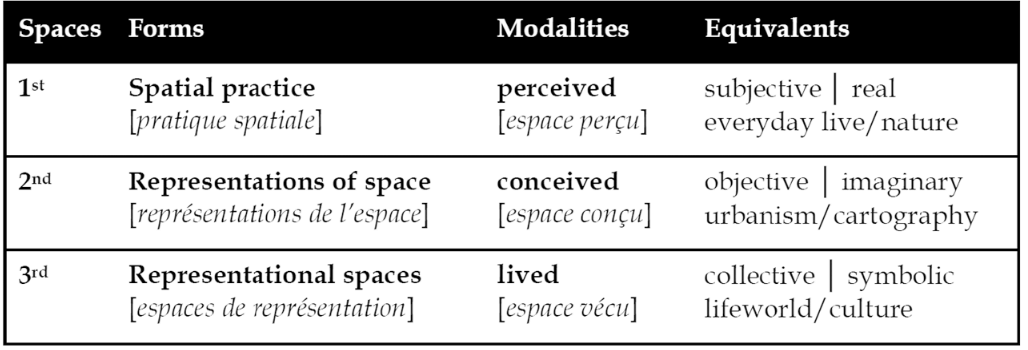
\includegraphics[width=0.75\linewidth]{c_3/lefebvretriad.png}}
    \caption[`Lefebvre's Triad of Spaces in (Günzel, 2019, p.14)']{`Lefebvre's Triad of Spaces in \citep[p. 14]{gunzel2019}'}\label{fig: lefebvretriad}
\end{figure}

Thus, de Certeau's distinction of space from place, whilst valuable insofar as it indicates the imbalance between human actors and institutions within the socio-cultural context - “the street, defined by urban planning is transformed into a space by walkers”, in itself is hardly a novel realisation. Furthermore, its fecundity diminishes with the assertion that this relation should be understood solely through a linguistic lens, i.e. the rules of “place” are written by those with power, and “space” is the result of actions by participants reading and interpreting those rules. To view the relation as such is to say that the actions of participants must within the diktat of place, and thus asserts that space originates in place and is therefore inseparable - "the only freedom you have is to formulate alternative sentences” \citep{vermeulen2015}. 

As Vermeulen further notes, for de Certeau, “space is an inter-subjective activation of a static site, a place”, whilst for Lefebvre, “place is the momentary suspension of a social flow, [a] space”. This leads to a contradiction in the formulation of “agency” as a concept: “de Certeau understands agency as the enactment of a script not our own, whereas Lefebvre sees it not as a container for action but as the construction of action itself.” 

It’s clear that with respect to 4EC approach to \textit{live} aesthetic experience it may be difficult to reconcile the 2nd and 3rd spaces of Lefebvre’s triad (conceived and lived), due to its own anti-representationalist standpoint. However oppositional on that front however, Lefebvre’s argument, through the prominence of social and class struggle under capitalism underpinning its formation, does indeed align itself with certain components (embodied, embedded) of enactivism: an approach that emphasises “the extended, intersubjective, and socially situated nature of cognitive systems” \citep[p. 6]{gallagher2017}: 
\begin{quote}
    “The relationship to space of a ‘subject’ who is a member of a group or society implies a certain relationship to [their] body and vice versa.” \cite[p. 40]{lefebvre1991}
\end{quote}
Additionally, Lefebvre’s “own particular brand of Marxism which stressed the importance of everyday life” \citep[p. 8]{merrifield1993} could be seen as aligned with Dewey’s own assertion of the importance of artwork to return “origin and operation” in everyday experience. In this way, the construction of 2nd and 3rd space doesn't necessarily have to fall fully under the remit of 4EC to explicate in real-time or live experience, rather, they may constitute the socio-cultural, and environmental aspects (norms, values, laws, traditions, and  conditions), as well as higher-order cognitive functions (meaning, and interpretation) that form the ‘environment’, as it is then to be experienced \textit{or} later considered by the enactive cogniser.

Thus, whereas ”the Metaverse” is somewhere to “show off your possessions”, and “maybe even” stage social interaction \citep{marr2022}, augmented space (or AR hybrid space) in contrast, prioritises the social, cultural, and aesthetic experience of the everyday. Architecture in “the Metaverse”, due to its origin in a capitalistic conception of society and technology, alienates its own inhabitants, since “under capitalism, it is only only through that [market] mediation that humans interact with buildings at all” \citep[p. 18]{mieville1998}. China Miéville’s critique here of physical architecture under capitalism could also be applied to the profit motivation for the commodity fetishisation of art in NFTs and the Metaverse. Not just ‘virtual land’, but digital art, music, video games, and social connection itself. More broadly, his “Marxist phenomenology” argues that to focus entirely on the physicality (of architecture in his text) is to “ignore the profound experiential ramifications” of living in a social system where such commodities are exchanged for profit. 

In stark contrast, architecture in augmented space consists in a constantly unfolding dialogue between humans and their environment, as perceptually guided by an ecosystem of hybrid processes; rather than consisting in alienation, and the “anxiety” induced by the commodity fetishism underlying capitalist profit motives. Application of Lefebvrian spatial theory indicates that AR can be a real force for social change, due to the way it can intervene spatially in the perception of participants, leading to new spatial characteristics and possibilites. When this is taken into action by people, either audiences, or performers, it puts the decision of when and where to "momentarily suspend" the social flow of space -- and thus construct "place" -- in their hands and in their bodies.

When Manifest.AR virtually trespassed the Museum of Modern Art (MoMA) with invisible and intangible AR art \citep{veenhof2010}; when \#OccupyAR broadcast the disembodied voices of geographically separated activists into Wall Street \citep{skwarek2018}; when Cem Kozar and Işıl Ünal \citeyearpar{thiel2011,thiel2018} revealed the unseen urban dynamics of the city of Istanbbul, it was through the live co-construction of new hybrid spaces — augmented spaces — that once hidden realities could be enacted anew. Whilst one might see parallels between these actions and what de Certeau terms “tactics”, the former, however, do more than just subverting place ‘proper’ through “alternative sentences” to borrow Vermeulen’s phrase. In actuality it is far more radical. Through the dynamic relations present in its hybridity — its incessant movement — emergent and novel states of self-organisation can occur within its constituents part(icipant)s. New socio-cultural meaning through sensory, perceptual and environmental modulation have the potential to synthesise from this ongoing process. In that spatiotemporal 'place' then, neither the MoMA nor Wall Street were themselves.

\section{Conclusion}\label{sec: theory-conclusion}
This chapter started with a grounding in the concept of 'art as experience', drawing from the work of \citep{dewey1934}. Dewey states that the capitalistic reverence of fine art, notably by the "nouveau riches", has led to art being put on a pedestal - disconnecting it from its origin and operation in the everyday experiences of people. Leddy and Puolakka have since proposed that "material of art should be from all sources and art should be accessible to all" \citeyearpar{leddy2021}. Dewey points towards the aesthetic experience that art entails, and notes that the "live creature" is inseparable from the environment in which they are embedded. Today, despite social media as a platform for cultural production of artisitic works has some merits, the fabric on which it is built is no different from the capitalist mechanisms that separated art from experience in the first place. Thus, open-source, hacker, DIY, and maker approaches were proposed as a method of democratising "all sources" of art, and attempting to increase accessibility. The focus on the body by Dewey also points towards the move towards tangible interface development, participatory design, and human-centered design.

To delve deeper into this experience of art, I propose an enactivist approach to considering cognition in experience. Often called 4E cognition (4EC), it states that cognitive process are embodied, embedded, enactive, and extended \citep{gallagher2017}. In considering the design, performance, and experience of AR, 4EC offers a fresh perspective on concepts such as agency, action, perception, immersion, and space.

The first theoretical lens through which to examine AR's design in computational art and music practice involved outlinined the importance of a complex systems framing of interface use and performance. I drew on existing research from the field of digital musical instrument design \citep{magnusson2009a,discipio2003,essl2006,armstrong2006,hayes2019,chevalier2018} in order to demonstrate the usefulness of considering performance systems as complex, and ecosystemic. Combining this theory with Schraffenberger's taxonomy of relationships between the virtual and real in AR, \citeyearpar{schraffenberger2018}, I developed the notion of "axes of conceptual distance", a loose framework by which to think about the (un)intentional design space that AR affords. The design of AR experiences could therefore be thought of as "invocation of a performance ecosystem constituted of relationships between real and virtual processes in the axes of spatial, thematic, material and ecological distance”. The section is ended on the assertion that despite these concepts, and Schraffenberger's relationship types being useful for the artist, they don't describe what happens in experience.

To examine what happens in the experience of participants, the second lens was one that took seriously the assertions of 4EC, namely that cognitive processes in experience are embodied, embedded, enactive and extended. I draw from multiple disciplines of similar theoretical and practical work in VR and AR to show how 4EC offers a novel framing by which to consider the experience of AR by participants, audiences, and performers. I refer back to Schraffenberger \citeyearpar{schraffenberger2018}, and outline multisensory examples of her "AR Subforms", and propose a set of key questions that may bring about new understandings of aesthetic experience in AR; e.g. \textit{"If a participant of an AR musical experience, or a performer of an AR musical instrument engages with this plurality of perceptual mediations, might the addition, removal, transformation, and completion of aspects of the environment have the potential to alter their own embodiment, relations to their environment, and enactive potential in specific areas of a space?"}

Closing out the trio of theoretical lenses, is a grounding of the aforementioned consequence of AR for the experience and construction of "space". I first critically examine the term "Metaverse" \citep{stephenson1992}. Its modern-day origin is in technologies like AR and VR, which in turn sprung from "deep within the military and Western - scientific - industrial - patriarchal complex" \cite{davies2004}, and its current operation has been heavily co-opted by crytocurrency projects. Because of this, in its current state, the "Metaverse" is hardly fertile ground for the "live creature" to experience art "accessibly", and from "all sources" \citep{dewey1934,leddy2021}, indeed, it mirrors the exact profit and exploitation motive of the historical context it originated in. I use the term "augmented space" \citep{manovich2006} to develop the proposition that R’s use as a medium for computational art and music could lead to the co-construction of new, hybrid spaces wherein novel, existing, hidden and suppressed realities can be acted out anew, and ground this in the social space theory of Henri Lefebvre \citeyearpar{lefebvre1991}, and of contemporary examples of AR activism \citep{veenhof2010,thiel2011,thiel2018,skwarek2018}.

In the next chapter I will outline the methodologies taken within my research, and draw links between historical and contemporary uses of AR, and the theoretical lenses I have proposed here.